\documentclass[12pt]{extarticle}
\usepackage{amsmath, amsthm, latexsym, tikz, graphicx, listings, microtype, mathtools, soul, color, fancyhdr}
\usepackage[margin=1in]{geometry}

\newenvironment{myindentpar}[1]%
 {\begin{list}{}%
         {\setlength{\leftmargin}{#1}}%
         \item[]%
 }
 {\end{list}}
 
\DeclarePairedDelimiter\abs{\lvert}{\rvert}%
\DeclarePairedDelimiter\norm{\lVert}{\rVert}%

% Swap the definition of \abs* and \norm*, so that \abs
% and \norm resizes the size of the brackets, and the 
% starred version does not.
\makeatletter
\let\oldabs\abs
\def\abs{\@ifstar{\oldabs}{\oldabs*}}
%
\let\oldnorm\norm
\def\norm{\@ifstar{\oldnorm}{\oldnorm*}}
\makeatother

\definecolor{lightgray}{gray}{0.65}
\definecolor{pinegreen}{RGB}{1, 171, 161}
\definecolor{lightblue}{RGB}{135, 206, 250}
\definecolor{dkgreen}{rgb}{0,0.6,0}
\definecolor{gray}{rgb}{0.5,0.5,0.5}
\definecolor{mauve}{rgb}{0.58,0,0.82}
\definecolor{darkblue}{rgb}{0.0,0.0,0.6}
\definecolor{cyan}{rgb}{0.0,0.6,0.6}

\newcommand*{\Value}{\frac{1}{2}x^2}%
\newcommand{\hlc}[2][yellow]{ {\sethlcolor{#1} \hl{#2}} }

\definecolor{codegray}{gray}{0.9}
\newcommand{\code}[1]{\colorbox{codegray}{\texttt{#1}}}

% /*--------------------------------------------------------------*/
%   Changing the values here sets the due date for the assignment!
% /*--------------------------------------------------------------*/
\newcommand{\duedate}{XX/XX/XX }
\newcommand{\semester}{SEMESTER}

\lstset{frame=tb,
  language=C++,
  breaklines=true,
  showstringspaces=false,
  columns=flexible,
  numbers=none,
  tabsize=3,
  escapeinside={(*@}{@*)}
  %,
  %commentstyle=\color{dkgreen},
  %stringstyle=\color{mauve}
}
\pagestyle{fancy}
\fancyhf{}
\renewcommand{\headrulewidth}{0pt}
\lhead{\color{lightgray} CSCE-313}
\rhead{\color{lightgray} \semester}
\rfoot{\thepage}
\pagenumbering{arabic}

\begin{document}

\begin{center}
    \underline{{\large Machine Problem 1: A High Performance Linked List \  }(Due: \duedate)}  \\
\end{center}


\ \\
{\large \underline{Introduction}:}

\begin{myindentpar}{6.5mm}

\ \\
In a traditional implementation of a linked list, memory is allocated for each newly inserted item.  When an item on this list is deleted, the memory allocated for it is freed and given back to the operating system.  Consequently, each allocation/de-allocation request for insertions or deletions respectively involves interacting with the operating system's memory manager.  System calls have a large overhead associated with them.  The processor must stop the execution of the user process, switch to executing system code, spend time performing the requested system function, and   As such, the calls to the memory manager hinder the performance of the linked list.  In this assignment, we will explore a solution to this problem which will produce a high performance and efficient implementation of a linked list.  

\ \\
In this assignment, the program you create will serve as the memory manager instead of relying on the operating system to do the dirty work.  Your program should obtain/reserve a fixed amount of memory from the operating system's memory manager during initialization (this is done by calling either malloc or new).  After initially acquiring memory from the system, your program should use this memory to manage the linked list throughout its execution.  Consequently, extraneous and expensive calls to the system's memory manager will no longer be necessary.  

\ \\
Each element of the linked list occupies a specific amount of space, known as the basic block size and denoted by the variable $b$.  The memory size as a whole is determined by the parameter $m$.  As such, there can be at most $m / b$ elements in the list.  Any insertion requests that would attempt to insert more than $m / b$ elements into the list should be immediately rejected.  

\ \\
The list should be managed through a Head Pointer (HP) and a Free Pointer (FP).  The former points to the head of the list, and the latter points to where the next insertion should happen.  

\ \\
Each linked list item can be separated into two sections: a header and a payload.  The header contains necessary information for maintaining the list (i.e. the next pointer, the previous pointer (for doubly linked lists), other metadata, etc...). The payload portion consists of a key-value pair.  The key is a 4 byte integer, and the value is of variable length, but has a maximum size that is determined by the header and key size.  

\ \\
Figure \#1 visually demonstrates how a singly linked list should be organized.  In the top of the figure, a linked list item is shown in detail.  Note that the size of pointers depend on the machine/OS type (i.e. in a 64-bit machine, pointers are 8-bytes as opposed to the 4-byte pointers present in 32-bit machines).  

\end{myindentpar}

\begin{center}
    Figure \#1: Structural view of a linked list in memory
\end{center}
\begin{center}
    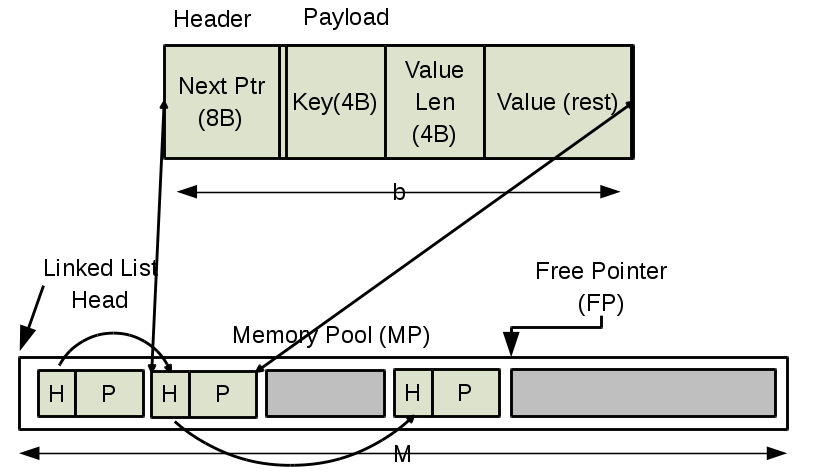
\includegraphics[scale=0.6]{ll_overview.png}
\end{center}

\ \\
{\large \underline{Assignment:}}

\begin{myindentpar}{6.5mm}

    \noindent
    \textbf{Part 1 - Singly-Linked List}

    \ \\
    You are to implement a singly-linked list with the mentioned features in either C or C++.  
    
    \begin{itemize}
        \setlength\itemsep{-0.05em}
    
        \item There should be three files in your program: main.c, linked\_list.h, and linked\_list.c.  A sample main file will be provided for you to finish.  
        \item Your implementation should contain at least the following functions (declared in the .h file and defined in the .c file).

\ \\
\vspace{-5mm}
\begin{lstlisting}[frame=single, language=C++]
Init(int M, int C)
(*@// Initially obtains M bytes of memory by calling the standard library function@*)
(*@// malloc() and initializes the linked list.  @*)

Destroy()
(*@// Destroys the linked list and returns memory to the system by calling another@*)
(*@// library function, free().@*)

Insert(int x, char* value_ptr, int value_len)
(*@// Inserts a key-value pair, where the key is an integer, x, and the value is some@*)
(*@// data pointed to by the pointer value\_ptr of length value\_len.  @*)
(*@// You should use the library function, memcpy() to copy the valu@*)
\end{lstlisting}
    
\begin{lstlisting}[frame=single, language=C++]
Delete(int x)
(*@// Deletes the first item from the beginning with the key x@*)

Lookup(int x)
(*@// Finds the given key in a list and returns a pointer to the@*)
(*@// first occurrence of that key@*)

PrintList()
(*@// Prints out all the items' key-value pairs sequentially starting from@*)
(*@// the head of the list.  Print only the key and the value-length@*)
(*@// Do not print the actual value as it could contain binary/non-printable data@*)
\end{lstlisting}
    
    \item Your implementation should include a program called testlist which reads the basic block size and the memory size (in bytes) from the command line, initializes the memory, makes some insertion/deletion calls, prints the list using the PrintList() function, and then destroys the allocated memory using Destroy().  Note that all these calls should go inside testlist's main function.  
    \item Use the getopt() C library function to parse the command line for arguments.  The usage for your program should be as follows:
    \begin{center}
        testlist [-b $<$blocksize$>$] [-s $<$memsize$>$]
    \end{center}
    
    \vspace{-5mm}
    \begin{displaymath}
        \begin{array}{|c|c|}
            \hline
            \text{-b $<$blocksize$>$} & \text{Defines the basic block size, b, in bytes.  Default = 128 bytes} \\
            \hline
            \text{-s $<$memsize$>$} & \text{Defines size of memory allocated in bytes.  Default = 512 kB} \\
            \hline
        \end{array}
    \end{displaymath}
    
    \item Make sure that your program does not crash in any case.  Here are a number of scenarios that your program should account for.  In these cases, your program should simply print an errir, skip the given instrution, and continue to work (i.e. do not exit for any reason).  
    \begin{itemize}
        \setlength\itemsep{-0.1em}
    
        \item Deleting non-existent keys from the list.  
        \item Trying to insert keys after the given memory is full.  
        \item Trying to insert values that do not fit in the payload section.  
        
    \end{itemize}
    
    \end{itemize}

    \ \\
    \textbf{Part 2 - Stratified Linked List}
    
    \ \\
    Modify the linked list you implemented in part 1 to make a multi-tiered list that groups keys into a number of disjoint intervals and keeps numbers from those intervals in separate lists.  Take another integer, $t$, ad input that indicates how many levels/tiers you will have in the tiered linked list.  Total memory, indicated by $M$, stays the same as in Part 1, which means that eacy tier now will contain M/t bytes of memory.  Each of these regions will act as an independent linked list as in Part 1.  
    
    \ \\
    In order to distribute numbers onto these separate linked lists, divide the integer number space (i.e. [0, $2^{31}$ - 1] or [0, INT\_MAX] for signed integers (Side note, the value INT\_MAX is contained in the header file: climits), you can safely assume that the input keys to your program are all non-negative) equally into t regions.  Note that you are only dividing the entire number space equally, and this division should not depend on the particular input array you are working with.  Therefore, it is possible that a particular input sequence could be placed into only one out of the t tiers simply because all the numbers in the sequence map to that tier.  However, if, in general, there is a uniform sample of input keys in the range of [0, INT\_MAX], then the tiers should contain roughly the same number of keys.  
    
    \ \\
    Figure 2 (shown below) demonstrates the organization of a 4-tier list.  All numbers in their $i$ should be less than those in tier $i + 1$.  You are NOT allowed to use the modulus operation on an input to determine its tier.  Instead, you should use either division or bit shift operations. The following are requirements of your program (Remember, like part 1, part 2 must be implemented in C or C++):
    
    \begin{itemize}
        \setlength\itemsep{-0.1em}

        \item There should be three files in your program: main.c, linked\_list2.h, and linked\_list2.c/cpp.  Similar to part1, a sample main file will be provided that includes some test cases for you to experiment with.  
        \item Provide implementations for all of the functions listed in part 1.  Note that those functions may work differently in the tiered design.  In some cases, the function arguments will also change.  For example, the Init(M, b) function will change to Init(M, b, t).  Furthermore, the PrintList function will change as well.  Do not print empty tiers (i.e. where no insertions have occurred).  
        \item Name your program testlist2, and this time, your program should accept the following command line arguments:
        
        \begin{center}
            testlist2 [-b $<$blocksize$>$] [-s $<$memsize$>$] [-t $<$tiers$>$]
        \end{center}
        \begin{center}
            Figure \#2: Organization of a tiered linked list
        \end{center}
        \begin{center}
            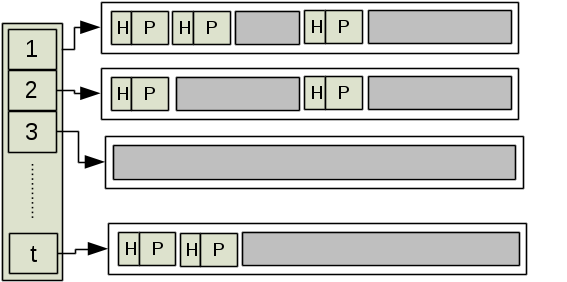
\includegraphics[scale=0.95]{tll_organization.png}
        \end{center}
        
    \end{itemize}
    
    \ \\
    \textbf{Report Documentation}
    \vspace{-3mm}
    
    \ \\
    Provide a PDF report describing your findings in both Parts 1 and 2.  You only have to write one report!  Do not write two separate reports for the two parts of this machine problem.  For part 1, do you notice any wastage of memory when items are deleted?  If so, can your program avoid such wastage?  How would you do so?  Can you think of a scenario where there is space in the memory but no insertion is possible?  What is the maximum size of the value when the pointers are 8 bytes?  For Part 2, derive a general expression for the range of numbers that go into the i-th tier of the list.  
    
    \ \\
    \textbf{Submission Instructions}
    
    \vspace{-3mm}
    \ \\
    Submit a zipped folder that contains two folders named MP1part1 and MP1part2, and a PDF report named MP1.pdf.  Both folders (MP1part1 and MP1part2) should contain 3 c/cpp/h files.  Demonstrate your work during lab meetings.  Make sure that your program runs on the CSE department's linux server (linux2.cse.tamu.edu).  Remember that we are using a new platform Vocareum (available at vocareum.com) for submitting machine problems.  Please register as a student on this website, play around with it, and become familiar with it so that there will be no issues before the assignment's deadline.  Please don't be afraid to talk to your TA or instructor if you have any issues.  
    

\end{myindentpar}


\end{document}